\scanpage{15}
% archive sheet number: 14
\margin{\handwritten{\figure{\begin{tikzpicture}\draw[gray] (0,.55) .. controls (.02,.35) and (.12,.15) .. (.2,.1);\draw[gray,densely dashed] (.43,.17) .. controls (.5,.38) and (.54,.62) .. (.58,.8);\end{tikzpicture}}}}
\uline{et transversal}.

 e) $\unsure{\mathbb{C}|\mathrm{C}}$ompatibilité avec \uline{changement de base} $S'\handwritten{\longrightarrow}S$, avec \uline{produits cartésiens} $Y_1\mathbin{\mathrm{x}}_S Y_2$ sur $S$.

\unsure{g|f}) Indépendance par rapport à $S$. \handwritten{($S\unsure{\text{---}|\longrightarrow}T$)}
\margin{\handwritten{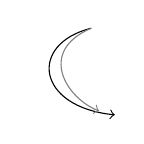
\begin{tikzpicture}\draw[->] (0,1.1) .. controls (-.8,.9) and (-.7,.1) .. (.3,0);\draw[gray,->] (0,1.1) .. controls (-.7,.8) and (-.3,.2) .. (.1,.05);\end{tikzpicture}}}

 f) Compatibilité avec changement d'anneau.

 h) \unsure{Remation|Relation} avec Gysin: Les classes (4.8),(4.9) s'interprètent comme l'image de $1_X$ par Gysin. Le transformé de (4.4) par $\mathrm{R}f_{\handwritten{!}}$, suivi de l'homomorphisme d'adjonction, est l'homomorphisme de Gysin.

Je pense que, compte tenu du formulaire de par.4, le formulaire \deleted{ici} proposé ici pour les classes fondamentales $\pm$ locales est pratiquement trivial\deleted{\unsure{,|e}} à partir des définitions. On peut \deleted{\unsure{don|donc}}, pour finir, récupérer un énoncé qui donne la \uline{caractérisation} des classes fondamentales locales dans le cas d'un couple lisse, par les propriétés suivantes 1) Nature locale (pour Zar suffit) 2) cas $p=0$ 3) cas $p=1$, quand $X$ est défini par une équation 4) propriété de cup-produit d) (où il suffit de \unsure{preddre|prendre} un des deux facteurs de codimension 1). Signaler\inserted{en remarque} que cet énoncé\deleted{\unsure{,}}\inserted{(existence et unicité d'une théorie des cl. fond. loc.)} peut se démontrer sans difficulté indépendamment de la théorie de dualité et de celle de l'homomorphisme trace, et avait été donnée dans le séminaire oral \deleted{\unsure{au prélimi|au prélim}} avant la dualité.

Remords: il serait pr\unsure{\.{u}|u}dent d'adjoindre au formulaire un
\margin{\handwritten{\begin{tikzpicture}\draw[->] (.3,0) .. controls (-1.4,2.4) and (-1.1,4.6) .. (.3,5.2);\draw (.4,.4)--(-.12,.1);\draw (-.12,.1) .. controls (-.8,-.8) and (-.6,-2.8) .. (-.7,-3.6) .. controls (-.7,-3.9) and (-.3,-3.9) .. (-.2,-3.9);\end{tikzpicture}}}

 i) On a commutativité dans le diagramme suivant
\diagram{\begin{tikzcd}[ampersand replacement=\&,column sep=3em,row sep=2em]
f^*(G)(\inserted{\handwritten{-}}p)\handwritten{[}\inserted{\handwritten{-}}2p\handwritten{]} \handwritten{\arrow[r]} \handwritten{\arrow[dr,bend right=18]} \& \mathrm{R}f^{\handwritten{!}}(G) \\
\& \mathrm{R}f^{\handwritten{!}}(A_Y)\overset{\underline{\mathrm{L}}}{\otimes}{\unsure{f|g}}^{\handwritten{*}}(G) \handwritten{\arrow[u]}
\end{tikzcd}},
où la flèche horizontale est (4.4), la flèche oblique est déduite par $\overset{\underline{\mathrm{L}}}{\otimes}G$ de (4.\unsure{5|9}),\deleted{dans le cas} et le flèche verticale est l'homomorphisme canonique qu'on devine,\deleted{et} analogue à celui de changement de base pour les \handwritten{$!$}, et qui manque dans 3.1\handwritten{(}tout comme ce dernier\handwritten{)}. On s'y intéressera sans doute surtout si $G$ est localement libre, donc l'homomorphisme en question est un isomorphisme.
